\documentclass[12pt]{article}
\usepackage{fullpage,graphicx,psfrag,url}
\usepackage[small,bf]{caption}
\setlength{\captionmargin}{30pt}

\input defs.tex
\newcommand{\sign}{\mathop{\bf sign}}

\bibliographystyle{alpha}

\title{Stochastic Subgradient Methods}
\author{Stephen Boyd and Almir Mutapcic\\
Notes for EE364b, Stanford University, Winter 2006-07}

\begin{document}
\maketitle

\section{Noisy unbiased subgradient}

Suppose $f:\reals^n \rightarrow \reals$ is a convex function.
We say that a random vector $\tilde g \in \reals^n$ is
a \emph{noisy (unbiased) subgradient} of $f$ at $x \in \dom f$ if
$g=\Expect \tilde g \in \partial f(x)$, \ie, we have
\[
f(z) \geq f(x)+ (\Expect \tilde g)^T(z-x)
\]
for all $z$.
Thus, $\tilde g$ is a noisy unbiased subgradient of $f$ at $x$
if it can be written as $\tilde g= g+v$, where $g \in \partial f(x)$ and
$v$ has zero mean.

If $x$ is also a random variable,
then we say that $\tilde g$ is a noisy subgradient of $f$ at $x$
(which is random) if
\[
\forall z \qquad f(z) \geq f(x)+ \Expect (\tilde g|x)^T(z-x)
\]
holds almost surely.
We can write this compactly as
$\Expect (\tilde g|x) \in \partial f(x)$.
(`Almost surely' is to be understood here.)

The noise can represent (presumably small) error in computing a true
subgradient, error that arises in Monte Carlo evaluation of a function
defined as an expected value, or measurement error.

Some references for stochastic subgradient methods
are~\cite[\S 2.4]{Sho:98}, \cite[Chap.\ 5]{Pol:87}.
Some books on stochastic programming in general
are~\cite{BiL:97,Pre:95,Mar:05}.

\section{Stochastic subgradient method}

The stochastic subgradient method is essentially the subgradient method,
but using noisy subgradients and a more limited set of step size rules.
In this context,
the slow convergence of subgradient methods helps us, since the
many steps help `average out' the statistical errors in the subgradient
evaluations.

We'll consider the simplest case, unconstrained
minimization of a convex function $f:\reals^n \rightarrow \reals$.
The stochastic subgradient method uses the standard update
\[
x^{(k+1)}=x^{(k)}-\alpha_k \tilde g^{(k)},
\]
where $x^{(k)}$ is the $k$th iterate, $\alpha_k > 0$ is the $k$th step
size, and $ \tilde g^{(k)} $ is a noisy subgradient of $f$ at $x^{(k)}$,
\[
\Expect (\tilde g^{(k)}|x^{(k)})  = g^{(k)} \in \partial f(x^{(k)}).
\]

Even more so than with the ordinary subgradient method,
we can have $f(x^{(k)})$ increase during the algorithm, so we keep
track of the best point found so far, and the associated function value
\[
f^{(k)}_\mathrm{best}  = \min\{f(x^{(1)}), \ldots, f(x^{(k)})\}.
\]
The sequences $x^{(k)}$, $\tilde g^{(k)}$, and $f^{(k)}_\mathrm{best}$
are, of course, stochastic processes.

\section{Convergence}

We'll prove a very basic convergence result for the stochastic
subgradient method, using step sizes that are square-summable but not summable,
\[
\alpha_k \geq 0, \qquad
\sum_{k=1}^\infty \alpha^2_k = \|\alpha\|_2^2< \infty,  \qquad
\sum_{k=1}^\infty \alpha_k = \infty.
\]
We assume there is an $x^\star$ that minimizes $f$, and
a $G$ for which $\Expect \|g^{(k)}\|_2^2 \leq G^2$
for all $k$.
We also assume that $R$ satisfies $\Expect \|x^{(1)}-x^\star\|_2^2 \leq
R^2$.

We will show that
\[
\Expect f^{(k)}_\mathrm{best} \rightarrow f^\star
\]
as $k \rightarrow \infty$, \ie, we have convergence in expectation.
We also have convergence in probability: for any $\epsilon> 0$,
\[
\lim _{k\rightarrow \infty} \Prob (f^{(k)}_\mathrm{best} \geq f^\star+
\epsilon) = 0.
\]
(More sophisticated methods can be used to show almost sure
convergence.)

We have
\BEAS
\Expect \left. \left( \|x^{(k+1)}-x^\star\|_2^2 \;\right|\; x^{(k)} \right)
&=& \Expect \left. \left( \|x^{(k)}-\alpha_k \tilde g^{(k)}-x^\star\|_2^2
\;\right|\; x^{(k)} \right) \\
&=& \|x^{(k)}-x^\star\|_2^2
	-2\alpha_k \Expect \left. \left( \tilde g^{(k)T}
(x^{(k)}-x^\star) \;\right|\; x^{(k)} \right)
	+\alpha_k^2\Expect \left. \left( \|\tilde g^{(k)} \|_2^2
\;\right|\; x^{(k)} \right) \\
&=& \|x^{(k)}-x^\star\|_2^2
	-2\alpha_k \Expect (\tilde g^{(k)} | x^{(k)})^T
(x^{(k)}-x^\star)
	+\alpha_k^2\Expect \left. \left( \|\tilde g^{(k)} \|_2^2
\;\right|\; x^{(k)} \right) \\
&\leq& \|x^{(k)}-x^\star\|_2^2
	-2\alpha_k (f(x^{(k)})-f^\star)+
\alpha_k^2 \Expect \left. \left( \|\tilde g^{(k)}\|_2^2
\;\right|\; x^{(k)} \right),
\EEAS
where the inequality holds almost surely, and follows because
$\Expect (\tilde g^{(k)}|x^{(k)}) \in \partial f(x^{(k)})$.

Now we take expectation to get
\[
\Expect \|x^{(k+1)}-x^\star\|_2^2
\leq \Expect \|x^{(k)}-x^\star\|_2^2
	    -2\alpha_k (\Expect f(x^{(k)})-f^\star)
	    +\alpha_k^2G^2,
\]
using $\Expect \|\tilde g^{(k)}\|_2^2 \leq G^2$.
Recursively applying this inequality yields
\[
\Expect \|x^{(k+1)}-x^\star\|_2^2 \leq
\Expect\|x^{(1)}-x^\star\|_2^2
-2\sum_{i=1}^k \alpha_i  (\Expect f(x^{(i)})-f^\star)
+G^2\sum_{i=1}^k \alpha_i^2.
\]
Using $\Expect \|x^{(1)}-x^\star\|_2^2 \leq R^2$,
$\Expect \|x^{(k+1)}-x^\star\|_2^2 \geq 0$, and $\sum_{i=1}^k \alpha_i^2
\leq \|\alpha \|_2^2$, we have
\[
2 \sum_{i=1}^k \alpha_i  (\Expect f(x^{(i)})-f^\star)
\leq R^2 +G^2\| \alpha \|_2^2.
\]
Therefore we have
\[
\min_{i=1,\ldots,k} (\Expect f(x^{(i)})-f^\star) \leq
\frac{R^2+G^2\|\alpha\|_2^2}{2 \sum_{i=1}^k \alpha_i},
\]
which shows that $\min_{i=1,\ldots,k} \Expect f(x^{(i)})$
converges to $f^\star$.

Finally, we note that
by Jensen's inequality and concavity of the minimum
function, we have
\[
\Expect f^{(k)}_\mathrm{best}
= \Expect \min_{i=1,\ldots,k} f(x^{(i)})
\leq \min_{i=1,\ldots,k} \Expect f(x^{(i)}),
\]
so $\Expect f^{(k)}_\mathrm{best}$ also converges to $f^\star$.

To show convergence in probability, we use
Markov's inequality to obtain, for $\epsilon>0$,
\[
\Prob(f^{(k)}_\mathrm{best} - f^\star \geq \epsilon) \leq
\frac{\Expect (f^{(k)}_\mathrm{best} - f^\star)}{\epsilon}.
\]
The righthand side goes to zero as $k \rightarrow \infty$, so
the lefthand side does as well.

\section{Example}

We consider the problem of minimizing a piecewise-linear function,
\[
\begin{array}{ll} \mbox{minimize} &
f(x) = \max_{i=1,\ldots,m} (a_i^T x + b_i),
\end{array}
\]
with variable $x \in \reals^n$.
At each step, we evaluate a noisy subgradient of the form
$\tilde g^{(k)} = g^{(k)} + v^{(k)}$, where $g^{(k)}\in \partial
f(x^{(k)})$ and $v^{(k)}$ are independent zero mean random variables.

We illustrate the stochastic subgradient method with the same
problem instance used in the notes on subgradient methods,
with $n=20$ variables, $m=100$ terms, and problem
problem data $a_i$ and $b_i$ generated from a unit normal
distribution.  We start with $x^{(1)}=0$,
and use the square summable but not summable step rule
$\alpha_k=1/k$.
To report $f(x^{(k)})-f^\star$,
we compute the optimal value~$f^\star$ using linear programming.

The noises $v^{(k)}$ are IID $\mathcal N(0,0.5I)$.
Since the norm of the vectors $a_i$ is on the order of $4$ or $5$
(the RMS value is $\sqrt{20}$), the subgradient noise is around
$25\%$ compared to the true subgradient.

Figure~\ref{f-pwl-error-fbest} shows the convergence
of the stochastic subgradient method
for two realizations of the noisy subgradient
process, together with the noise-free case for comparison.
This figure shows that convergence is only a bit slower with
subgradient noise.

We carried out $100$ realizations, and show the (sample)
mean and standard
deviation of $f_\mathrm{best}^{(k)} - f^\star$ for $k$ in multiples
of $250$, in figure~\ref{f-pwl-error-fbest-avg}.
(The error bars show the mean plus and minus one standard deviation.)
Figure~\ref{f-pwl-error-fbest-dist} shows
the empirical distribution
(over the $100$ realizations) of
$f_\mathrm{best}^{(k)} - f^\star$ at
iterations $k=250$, $k=1000$, and $k=5000$.

\begin{figure}
\begin{center}
\psfrag{k}[t][b]{$k$}
\psfrag{fbest - fmin}[b][t]{$f_\mathrm{best}^{(k)} - f^\star$}
\psfrag{noise-free realize}{noise-free case}
\psfrag{realize1}{realization 1}
\psfrag{realize2}{realization 2}
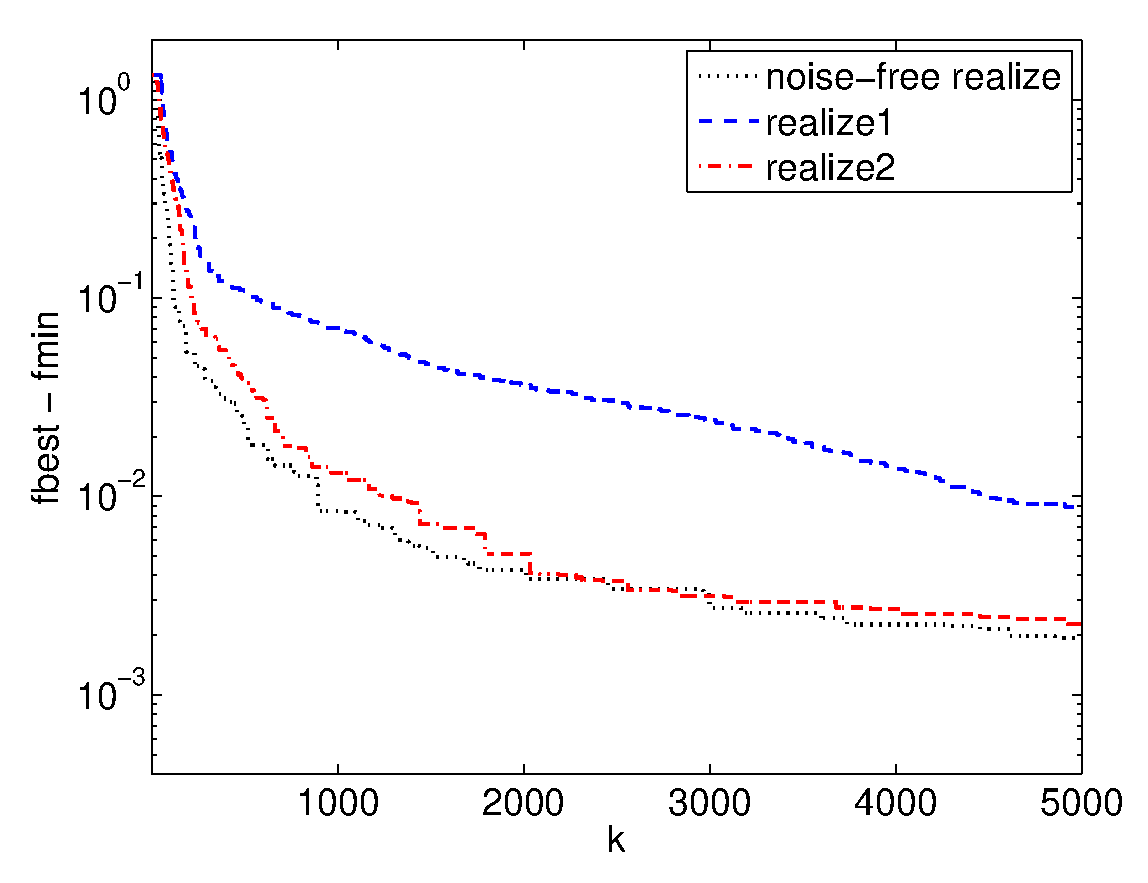
\includegraphics[width=0.6\textwidth]{matlab/pwl_error_fbest_realize}
\end{center}
\caption{The value of $f_\mathrm{best}^{(k)} - f^\star$
versus iteration number~$k$,
for the subgradient method with step size
$\alpha_k=1/k$. The plot shows a noise-free realization,
and two realizations with subgradient noise.}
\label{f-pwl-error-fbest}
%\end{figure}
%
%\begin{figure}
\begin{center}
\psfrag{k}[t][b]{$k$}
\psfrag{average fbest - fmin}[b][t]
{$\Expect f_\mathrm{best}^{(k)} - f^\star$}
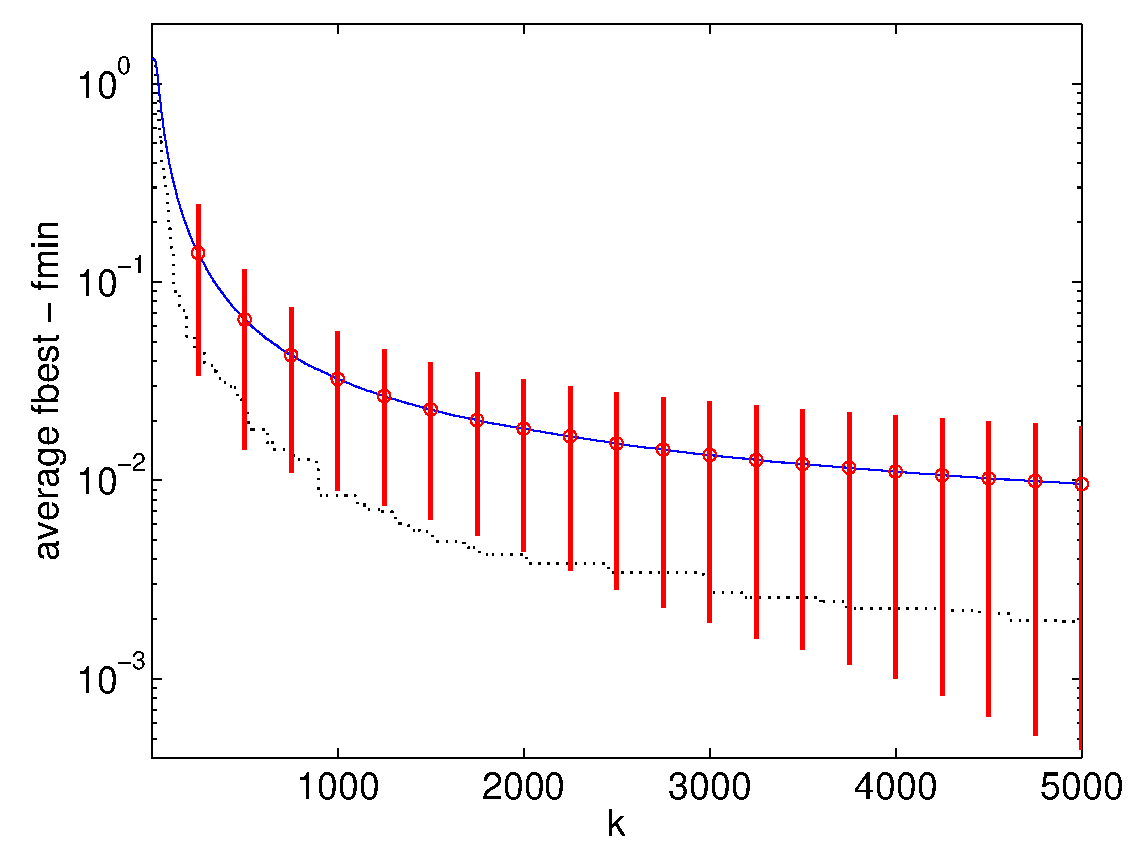
\includegraphics[width=0.6\textwidth]{matlab/pwl_error_fbest_average}
\end{center}
\caption{Average and one standard deviation error bars
for $f_\mathrm{best}^{(k)} - f^\star$ versus iteration number~$k$,
computed using $100$ realizations, every $250$ iterations.}
\label{f-pwl-error-fbest-avg}
\end{figure}

\begin{figure}
\begin{center}
\psfrag{iter 250}[c][b]{$k=250$}
\psfrag{iter 1000}[c][b]{$k=1000$}
\psfrag{iter 5000}[c][b]{$k=5000$}
\psfrag{average fbest - fmin}[b][t]
{$\Expect f_\mathrm{best}^{(k)} - f^\star$}
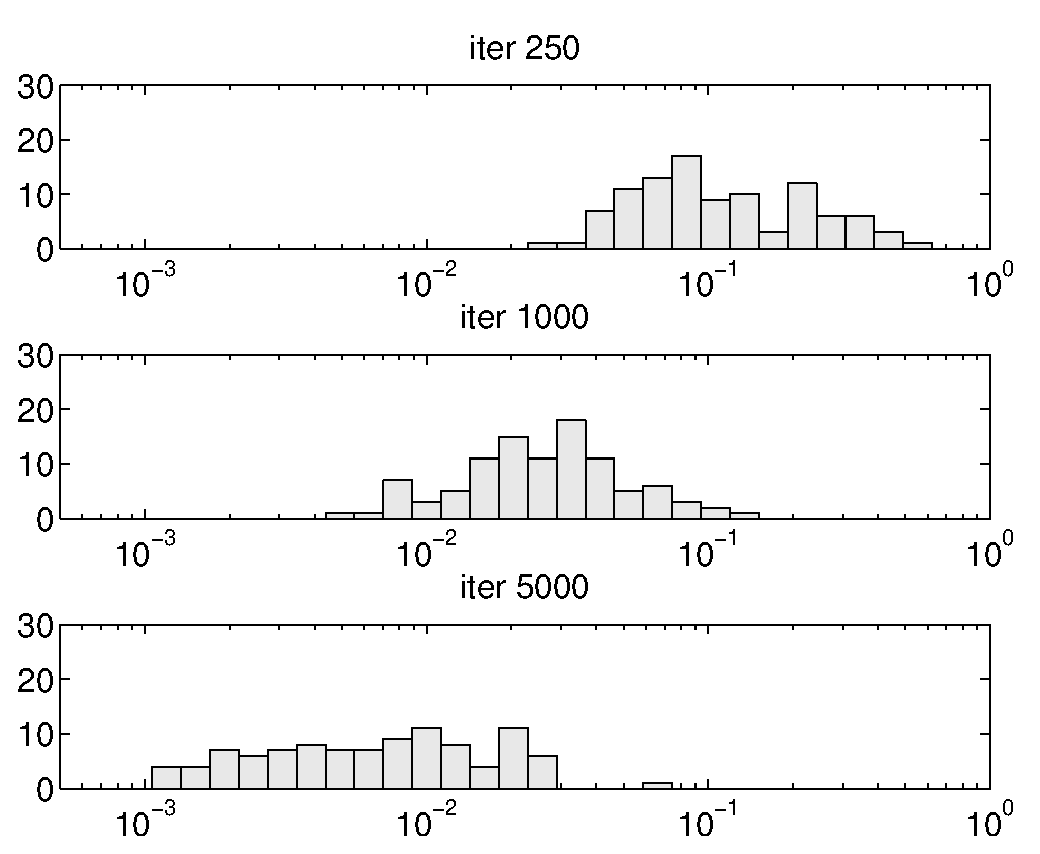
\includegraphics[width=0.7\textwidth]{matlab/pwl_error_fbest_dist}
\end{center}
\caption{Empirical distributions of
$f_\mathrm{best}^{(k)} - f^\star$
at $k=250$, $k=1000$, and $k=5000$ iterations, based on
$100$ realizations.}
\label{f-pwl-error-fbest-dist}
\end{figure}

\clearpage
\section{Stochastic programming}

A stochastic programming problem has the form
\BEQ\label{e-stoch-prog}
\begin{array}{ll}
\mbox{minimize} & \Expect f_0(x,\omega)\\
\mbox{subject to} & \Expect f_i(x,\omega) \leq 0, \quad i=1, \ldots, m,
\end{array}
\EEQ
where $x \in \reals^n$ is the optimization variable, and $\omega$ is
a random variable.
If $f_i(x,\omega)$ is convex in $x$ for each $\omega$, the problem
is a convex stochastic programming problem.
In this case the objective and constraint functions are convex.

Stochastic programming can be used to model a variety of robust
design or decision problems with uncertain data.
Although the basic form above involves only expectation or average
values, some tricks can be used to capture other measures of the
probability distributions of $f_i(x,\omega)$.
We can replace an objective or constraint term $\Expect f(x,\omega)$
with $\Expect \Phi(f(x,\omega))$, where $\Phi$ is a convex increasing
function.
For example, with $\Phi(u)=\max(u,0)$, we can form a constraint
of the form
\[
\Expect f_i(x,\omega)_+ \leq \epsilon,
\]
where $\epsilon$ is a positive parameter, and $(\cdot)_+$ denotes
positive part.
Here $\Expect f_i(x,\omega)_+$ has a simple interpretation as
the \emph{expected violation} of the $i$th constraint.
It's also possible to combine the constraints, using a single
constraint of the form
\[
\Expect \max(f_1(x,\omega)_+, \ldots, f_m(x,\omega)_+) \leq \epsilon.
\]
The lefthand side here can be interpreted as the \emph{expected
worst violation} (over all constraints).

Constraints of the form $\Prob(f_i(x,\omega) \leq 0) \geq \eta$,
which require a constraint to hold with a probability
(or reliability) exceeding $\eta$,
are called \emph{chance constraints}.  These constraints
cannot be directly handled using the simple trick above, but an expected
violation constraint can often give a good approximation for a chance
constraint. (Some chance constraints can be handled exactly, \eg,
when $f(x,\omega)=(a+\omega)^Tx-b$, $\omega$ is Gaussian,
and $\eta \geq 0.5$.)

Recall that Jensen's inequality tells us
\[
\Expect f_i(x,\omega) \geq f_i(x,\Expect \omega).
\]
Now consider the problem
\BEQ\label{e-unc-equ}
\begin{array}{ll}
\mbox{minimize} & f_0(x, \Expect \omega)\\
\mbox{subject to} & f_i(x, \Expect \omega) \leq 0,
\quad i=1, \ldots, m,
\end{array}
\EEQ
obtained by replacing the random variable in each function by its
expected value.
This problem is sometimes called the \emph{certainty equivalent}
of the original stochastic programming problem~(\ref{e-stoch-prog}),
even though they are equivalent only in very special cases.
By Jensen's inequality, the constraint set for the uncertainty
equivalent problem is
larger than the original stochastic problem~(\ref{e-stoch-prog}),
and its objective is smaller.
It follows that the optimal value of the uncertainty equivalent
problem gives a lower bound on the optimal value of the
stochastic problem~(\ref{e-stoch-prog}).
(It can be a poor bound, of course.)

\subsection{Noisy subgradient of expected function value}

Suppose $F: \reals^n \times \reals^ p \rightarrow \reals$, and
$F(x,w)$ is convex in $x$ for each $w$.
We define
\[
f(x) = \Expect F(x,w) = \int F(x,w) p(w) \; dw,
\]
where $p$ is the density of $w$.  (The integral is in $\reals^p$.)
The function $f$ is convex.
We'll show how to compute a noisy unbiased subgradient of $f$ at $x$.

The function $f$ comes up in many applications. We can think of $x$
as some kind of design variable to be chosen, and $w$ as some kind of
parameter that is random, \ie, subject to statistical fluctuation.
The function $F$ tells us the cost of choosing $x$ when $w$ takes
a particular value; the function $f$, which is deterministic,
gives the average cost of choosing $x$, taking the statistical
variation of $w$ into account.
Note that the dimension of $w$, how it enters $F$, and the
distribution are not restricted; we only require
that for each value of $w$, $F$ is convex in $x$.

Except in some very special cases, we cannot easily compute $f(x)$
exactly.  However, we can approximately compute $f$ using Monte Carlo
methods, if we can cheaply generate samples of $w$
from its distribution.  (This depends on the distribution.)
We generate $M$ independent samples $w_1, \ldots, w_M$, and then take
\[
\hat f(x) = \frac{1}{M} \sum_{i=1}^M F(x,w_i)
\]
as our estimate of $f(x)$.  We hope that if $M$ is
large enough, we get a good estimate.
In fact, $\hat f(x)$ is a
random variable with $\Expect \hat f(x) = f(x)$, and a
variance equal to $c/M$, where $c$ is the variance of $F(x,\omega)$.
If we know or bound $c$, then we can at least bound the probability
of a given level of error, \ie,
$\Prob (|\hat f(x) - f(x)| \geq \epsilon)$.
In many cases it's possible to carry out a much more sophisticated
analysis of the error in Monte Carlo methods, but we won't pursue that
here.
A summary for our purposes is:
we cannot evaluate $f(x)$ exactly, but we can get
a good approximation, with (possibly) much effort.


Let $G: \reals^n \times
\reals^p \rightarrow \reals^n$ be a function that satisfies
\[
G(x,w) \in \partial_x F(x,w)
\]
for each $x$ and $w$.
In other words, $G(x,w)$ selects a subgradient for each
value of $x$ and $w$.  If $G(x,w)$ is differentiable in $x$
then we must have $G(x,w)=\nabla _xF(x,w)$.

We claim that
\[
g=\Expect G(x,w) = \int G(x,w) p(w) \; dw \in \partial f(x).
\]
To see this, note that for each $w$ and any $z$ we have
\[
F(z,w) \geq F(x,w) + G(x,w)^T(z-x),
\]
since $G(x,w) \in \partial_x F(x,w)$.
Multiplying this by $p(w)$, which is nonnegative, and integrating
gives
\BEAS
\int F(z,w)p(w)\; dw &\geq&
\int \left( F(x,w) + G(x,w)^T(z-x) \right) p(w) \; dw\\
& = &
f(x) + g^T(z-x).
\EEAS
Since the lefthand side is $f(z)$, we've shown $g \in \partial f(x)$.

Now we can explain how to compute a noisy unbiased
subgradient of $f$ at $x$.
Generate independent samples $w_1, \ldots, w_M$.
We then take
\[
\tilde g = \frac{1}{M} \sum_{i=1}^M G(x,w_i).
\]
In other words, we evaluate a subgradient of $f$, at $x$, for
$M$ random samples of $w$, and take $\tilde g$ to be the average.
At the same time we can also compute $\hat f(x)$, the Monte
Carlo estimate of $f(x)$.
We have $\Expect \tilde g = \Expect G(x,w) =g$, which we showed
above is a subgradient of $f$ at $x$.  Thus, $\tilde g$ is a noisy
unbiased sugradient of $f$ at $x$.

This result is independent of $M$.  We can even take $M=1$. In
this case, $\tilde g = G(x,w_1)$.  In other words, we simply
generate \emph{one} sample $w_1$ and use the subgradient of
$F$ for that value of $w$. In this case $\tilde g$ could hardly
be called a good approximation of a subgradient of $f$, but its
mean is a subgradient, so it is a valid noisy unbiased subgradient.

On the other hand, we can take $M$ to be large.  In this case,
$\tilde g$ is a random vector with mean $g$ and very small variance,
\ie, it is a good estimate of $g$, a subgradient of $f$ at $x$.

\subsection{Example}

We consider the problem of minimizing the expected value
of a piecewise-linear convex function with random coefficients,
\[
\begin{array}{ll} \mbox{minimize} &
f(x) = \Expect \max_{i=1,\ldots,m} (a_i^T x + b_i),
\end{array}
\]
with variable $x \in \reals^n$.
The data vectors $a_i \in \reals^n$ and $b_i \in \reals$
are random with some given distribution.
We can compute an (unbiased) approximation of $f(x)$, and a
noisy unbiased subgradient $g \in \partial f(x)$, using
Monte Carlo methods.

We consider
a problem instance with $n=20$ variables and $m=100$ terms.
We assume that $a_i \sim \mathcal{N}(\bar a_i, 5 I)$
and $b \sim \mathcal{N}(\bar b, 5 I)$.
The mean values $\bar a_i$ and $\bar b$ are generated
from unit normal distributions (and are the same as the constant
values used called $a_i$ and $b_i$ in previous examples).
We take $x^{(1)}=0$ as the starting point
and use the step size rule $\alpha_k=1/k$.

We first compare the solution of the
stochastic problem~$x_\mathrm{stoch}$ (obtained from the
stochastic subgradient method) with $x_\mathrm{ce}$,
the solution of the certainty equivalent problem
\[
\begin{array}{ll} \mbox{minimize} &
f_\mathrm{ce} (x)
= \max_{i=1,\ldots,m} (\Expect a_i^T x +  \Expect b_i)
\end{array}
\]
(which is the same piecewise-linear minimization problem
considered in earlier examples).
We also compare it with $x_\mathrm{heur}$,
the solution of the problem
\[
\begin{array}{ll} \mbox{minimize} &
f_\mathrm{heur} (x)
= \max_{i=1,\ldots,m} (\Expect a_i^T x +  \Expect b_i +
\lambda \|x\|_2),
\end{array}
\]
where $\lambda$ is a positive parameter.
The extra terms are meant to account for the variation in $a_i^Tx+b$
caused by variation in $a_i$; the problem above can be cast as an SOCP
and easily solved.
We chose $\lambda = 1$, after some experimentation.

The certainty equivalent values for the three points are
$f_\mathrm{ce}(x_\mathrm{ce}) = 1.12$,
$f_\mathrm{ce}(x_\mathrm{heur}) = 1.23$, and
$f_\mathrm{ce}(x_\mathrm{stoch}) = 1.44$.
We (approximately) evaluate $f(x)$ for these three points,
based on $1000$ Monte Carlo samples, obtaining
$f(x_\mathrm{ce}) \approx 2.12$,
$f(x_\mathrm{heur}) \approx 1.88$, and
$f(x_\mathrm{stoch}) \approx 1.83$.
The empirical distributions of $\max_i (a_i^T x + b_i)$,
for $x=x_\mathrm{stoch}$, $x = x_\mathrm{heur}$, and
for $x=x_\mathrm{ce}$,
are shown in figure~\ref{f-stoch-pwl-fbest-dist}.

In summary, the heuristic finds a point that is good, but not
quite as good as the stochastic optimal.
Both of these points are much better than the certainty equivalent
point.

\begin{figure}
\begin{center}
\psfrag{nominal}[c][b]{$x_\mathrm{ce}$}
\psfrag{heuristic}[c][b]{$x_\mathrm{heur}$}
\psfrag{K = 100}[c][b]{$x_\mathrm{stoch}$}
\psfrag{nom mean}{$f(x_\mathrm{ce})$}
\psfrag{nom nom}{}
\psfrag{heur mean}{$f(x_\mathrm{heur})$}
\psfrag{heur nom}{}
\psfrag{k100 mean}{$f(x_\mathrm{stoch})$}
%\psfrag{k100 mean}{}
%\psfrag{k100 nom}{$f_\mathrm{ce}(x_\mathrm{stoch})$}
\psfrag{k100 nom}{}
\psfrag{average fbest - fmin}[b][t]
{$\Expect f_\mathrm{best}^{(k)} - f^\star$}
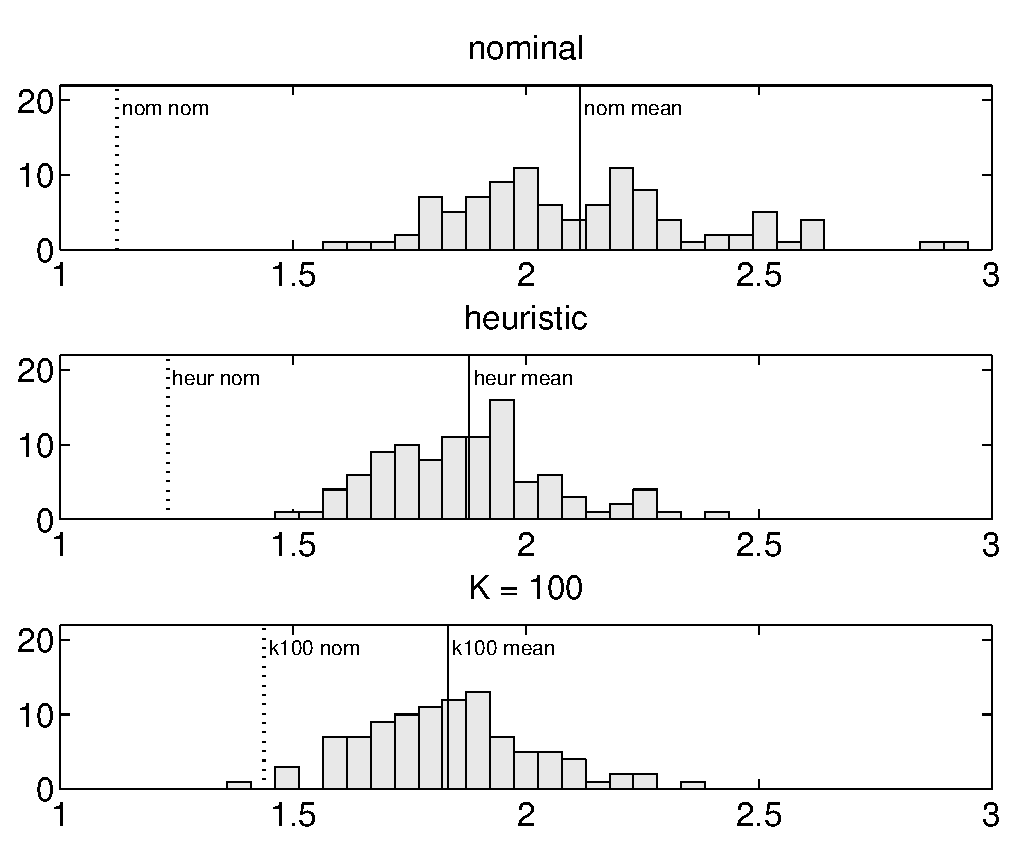
\includegraphics[width=0.7\textwidth]{matlab/expected_pwl_fbest_dist}
\end{center}
\caption{Empirical distributions of
$\max_i (a_i^Tx + b_i)$ for the certainty equivalent solution
$x_\mathrm{ce}$, heuristic-based solution $x_\mathrm{heur}$,
and the stochastic optimal solution $x_\mathrm{stoch}$.
The dark lines show the value of $f(x)$, and the dotted lines
show the value of $f_\mathrm{ce}(x)$.
}
\label{f-stoch-pwl-fbest-dist}
\end{figure}

Now we show the convergence of the stochastic subgradient method,
evaluating noisy subgradients with $M=1$, $M=10$, $M=100$, and
$M=1000$ samples at each step.
For $M=1000$, we are computing a fairly accurate subgradient; for
$M=1$, the variance in our computed subgradient is large.

We (approximately) evaluate
the function $f(x)$ using $M=1000$ samples at each iteration,
and keep track of the best value $f^{(k)}_\mathrm{best}$.
We estimate $f^\star$
by running the stochastic subgradient algorithm for a large
number of iterations.
Figure~\ref{f-stoch-pwl-fbest} shows the convergence
for one realization for each of the four values of $M$.
As expected, convergence is faster with $M$ larger, which yields
a more accurate subgradient.
Assuming the cost of an iteration is proportional to $M$,
$M=1$ seems to be the best choice.
In any case, there seems little advantage (at least
in this example) to using a value of $M$ larger than $10$.

\begin{figure}
\begin{center}
\psfrag{k}[t][b]{$k$}
\psfrag{fbest - fmin}[b][t]{$f_\mathrm{best}^{(k)} -\hat f^\star$}
\psfrag{K = 1}{$M=1$}
\psfrag{K = 10}{$M=10$}
\psfrag{K = 100 label}{$M = 100$}
\psfrag{K = 1000}{$M = 1000$}
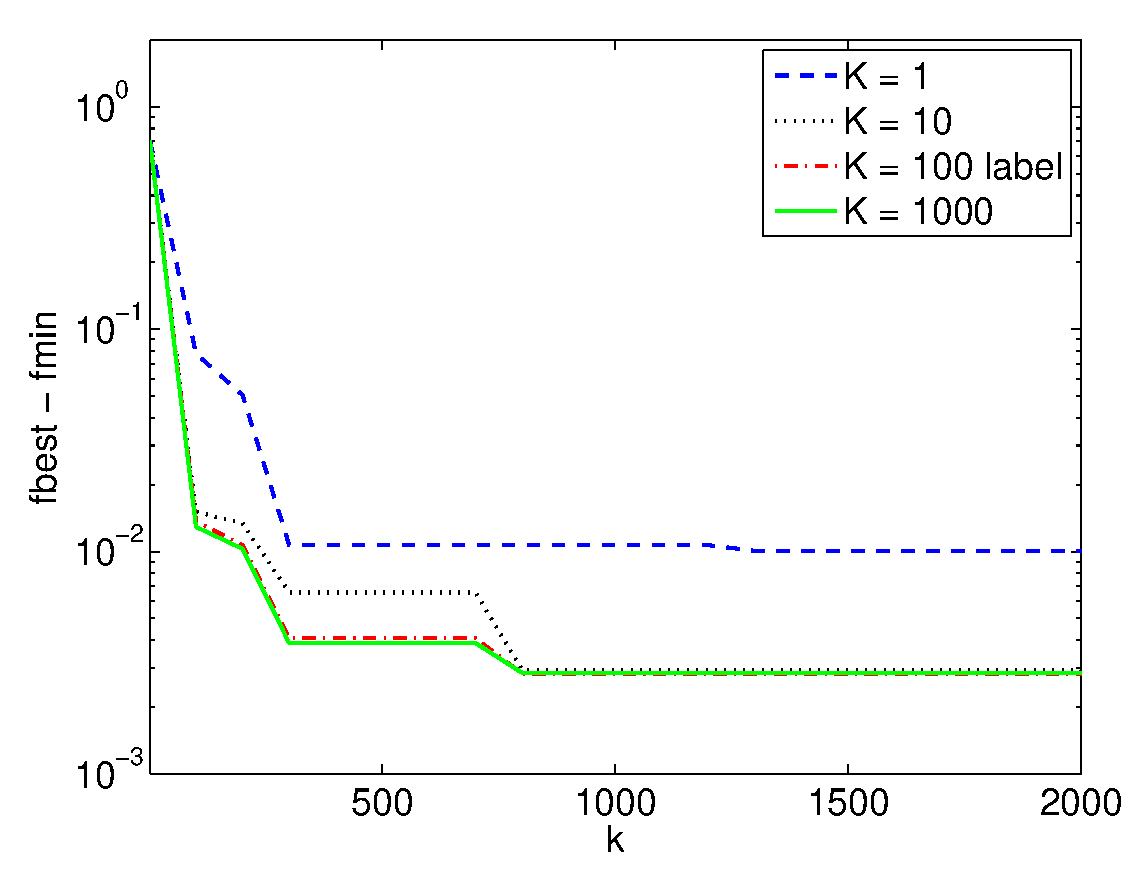
\includegraphics[width=0.6\textwidth]{matlab/expected_avgpwl_fbest}
\end{center}
\caption{The value of $f_\mathrm{best}^{(k)} - f^\star$
versus iteration number~$k$, for the stochastic subgradient method
with step size rule $\alpha_k=1/k$.
The plot shows one realization for noisy subgradients  evaluated
using $M=1$, $M=10$, $M=100$, and $M=1000$.}
\label{f-stoch-pwl-fbest}
\end{figure}

\section{More examples}

%\subsection{Optimal stocking}
%
%amount of stock is variable $x \in \reals^n$
%
%$x \succeq 0$, $x \preceq x_\mathrm{max}$.
%
%demand $\in \reals^n$ is unknown, statistical. $x \succeq 0$
%
%amount sold is $\min(x,d)$

\subsection{Minimizing expected maximum violation}

The vector $x \in \reals^n$ is to be chosen subject to some
(deterministic) linear inequalities $Fx \preceq g$.
These can represent manufacturing limits, cost limits, etc.
Another set of \emph{random} inequalities is given as $Ax \preceq b$,
where $A$ and $b$ come from some distribution.
We would like these inequalities to hold, but because $A$ and $b$
vary, there may be no choice of $x$ that results in
$Ax \preceq b$ almost surely.
We still would like to choose $x$ so that $Ax \preceq b$ holds often,
and when it is violated, the violation is small.

Perhaps the most natural problem formulation is to maximize the yield,
defined as $\Prob (Ax \preceq b)$.  In some very special cases
(\eg, $A$ is deterministic and $b$ has log-concave density),
this can be converted to a convex problem; but in general it is
not convex.
Also, yield is not sensitive to how much the inequalities
$Ax \preceq b$ are violated; a small violation is the same as a large
variation, as far as the yield is concerned.

Instead, we will work with the \emph{expected maximum violation}
of the inequalities.
We define the \emph{maximum violation} as
\[
\max((Ax-b)_+)= \max_i (a_i^Tx-b)_+,
\]
where $a_i$ are the rows of $A$.
The maximum violation is zero if and only if
$Ax \preceq b$; it is positive otherwise.
The expected violation is
\[
\Expect \max((Ax-b)_+)=
\Expect \left(\max_i (a_i^Tx-b_i)_+ \right).
\]
It is a complicated
but convex function of $x$, and gives a measure of how often, and by
how much, the constraints $Ax \preceq b$ are violated.
It is convex no matter what the distribution of $A$ and $b$ is.

As an aside, we note that
many other interesting measures of violation could also be used,
such as the expected total (or average) violation,
$\Expect \ones^T(a_i^Tx-b_i)_+$,
or the expected sum of the squares of the individual violations,
$\Expect \| (Ax-b)_+\|_2^2$.
We can even measure violation by the expected distance from the desired
polyhedron, $\Expect \dist (x, \{z \;|\; Az \preceq b\})$,
which we call the expected violation distance.

Back to our main story, and using expected (maximum) violation,
we have the problem
\[
\begin{array}{ll}
\mbox{minimize} & \Expect \max((Ax-b)_+) =
\Expect \left(\max_i (b_i-a_i^Tx)_+ \right)\\
\mbox{subject to} & Fx \preceq g.
\end{array}
\]
The data are $F$, $g$, and the distribution of $A$ and $b$.

We'll use a stochastic projected subgradient method to solve
this problem.
Given a point $x$ that satisfies $Fx \preceq g$, we need to
generate a noisy unbaised subgradient $\tilde g$ of the objective.
To do this we first
generate a sample of $A$ and $b$.
If $Ax \preceq b$, we can take $\tilde g=0$.
(Note: if a subgradient is zero, it means we're done; but that's not
the case here.)
In the stochastic subgradient algorithm,
$\tilde g=0$ means we don't update
the current value of $x$.  But we don't stop the algorithm,
as we would in a deterministic projected subgradient method.

If $Ax \preceq b$ is violated, choose $j$ for which
$b_j-a_j^Tx= \max_i (b_i-a_i^Tx)_+$.  Then we can take $\tilde g
= a_j$.  We then set $x_\mathrm{temp}=x-\alpha_k a_j$,
where $\alpha_k$ is the step size.
Finally, we project $x_\mathrm{temp}$ back to the feasible set
to get the updated value of $x$.  (This can be done by solving a QP.)

We can generate a number of samples of $A$ and $b$, and use the
method above to find an unbiased noisy subgradient for each case.
We can use the average of these as $\tilde g$.
If we take enough samples, we can simultaneously estimate
the expected maximum violation for the current value of $x$.

A reasonable starting point is a point well inside the certainty
equivalent inequalities $\Expect A x \preceq \Expect b$,
that also satisfies $F x \preceq g$.
Simple choices include the analytic, Chebyshev, or maximum
volume ellipsoid centers, or the point that maximizes the margin
$\max (b-Ax)$, subject to $Fx \preceq g$.

\subsection{On-line learning and adaptive signal processing}

We suppose that $(x,y) \in \reals^n \times \reals$ have
some joint distribution.  Our goal is to find a weight vector $w \in
\reals^n$ for which $w^Tx$ is a good estimator of $y$.
(This is linear regression; we can
add an extra component to $x$ that is always one to get an
affine estimator of the form $w^Tx+v$.)
We'd like to choose a weight vector that minimizes
\[
J(w) = \Expect l(w^Tx-y),
\]
where $l:\reals \rightarrow \reals$ is a convex \emph{loss function}.
For example, if $l(u)=u^2$, $J$ is the mean-square error;
if $l(u)=|u|$, $J$ is the mean-absolute error.
Other interesting loss functions include the Huber function,
or a function with dead zone, as in $l(u)=\max\{|u|-1,0\}$.
For the special case $l(u)=u^2$, there is an analytic formula for
the optimal $w$, in terms of the mean and covariance matrix of
$(x,y)$.  But we consider here the more general case.
Of course $J$ is convex, so minimizing $J$ over $w$ is a
convex optimization problem.

We consider an on-line setting, where we do not know the distribution
of $(x,y)$.  At each step (which might correspond to time, for example),
we are given a sample $(x^{(i)},y^{(i)})$ from the distribution.
After $k$ steps, we could use the $k$ samples to estimate the
distribution; for example, we could choose $w$ to minimize
the average loss under the empirical distribution.
This approach requires that we store all past samples, and we need to
solve a large problem each time a new sample comes in.

Instead we'll use the stochastic subgradient method, which is really
simple.  In particular, it requires essentially no storage (beyond the
current value of $w$), and very little computation.
The disadvantage is that it is slow.

We will carry out a stochastic subgradient step each time a new
sample arrives.
Suppose we are given a new sample $(x^{(k+1)},y^{(k+1)})$,
and the current weight value is $w^{(k)}$.
Form
\[
l'(w^{(k)T}x^{(k+1)}-y^{(k+1)})x^{(k+1)},
\]
where $l'$ is the derivative of $l$.  (If $l$ is nondifferentiable,
substitute any subgradient of $l$ in place of $l'$.)
This is a noisy unbiased subgradient of $J$.

Our on-line algorithm is very simple: when $(x^{(k+1)},y^{(k+1)})$
becomes available, we update $w^{(k)}$ as follows:
\BEQ\label{e-online-update}
w^{(k+1)}=w^{(k)}-\alpha_k
l'(w^{(k)T}x^{(k+1)}-y^{(k+1)})x^{(k+1)}.
\EEQ
Note that $w^{(k)T}x^{(k+1)}-y^{(k+1)}$ is the
prediction error for the $k+1$ sample, using the weight from
step $k$.
We can choose (for example) $\alpha_k=1/k$.

In signal processing, updates of the form~(\ref{e-online-update})
are widely used in \emph{adaptive signal processing}, typically with
$l(u)=u^2$.
In this case the update~(\ref{e-online-update}) is called
the \emph{LMS} (least mean-square) algorithm.

We illustrate the method with a simple example with $n=10$,
with $(x,y) \sim \mathcal N(0,\Sigma)$, where $\Sigma$ is chosen
randomly, and $l(u)=|u|$. (For the problem instance,
we have $\Expect( y^2 ) \approx 12$.)
The update has the simple form
\[
w^{(k+1)}=w^{(k)}-\alpha_k
\sign (w^{(k)T}x^{(k+1)}-y^{(k+1)})x^{(k+1)}.
\]
We take $\alpha_k=1/k$.
(In adaptive signal processing, this is called
a \emph{sign algorithm}.)

We compute $w^\star$ using the stochastic subgradient algorithm,
which we run for $5000$ iterations.
%and we compare it to $w^\mathrm{lms}$, the weight
%that minimizes mean-square error.
Figure~\ref{f-online-reg-errors} shows the behaviour of the
prediction error $w^{(k)T}x^{(k+1)}-y^{(k+1)}$
for the first $300$ iterations of the run.
Figure~\ref{f-online-reg-dist} shows the empirical distibution
(over the $1000$ realizations) of the prediction errors for $w^\star$.

\begin{figure}
\begin{center}
\psfrag{pred error}[b][t]{prediction error}
\psfrag{k}[t][b]{$k$}
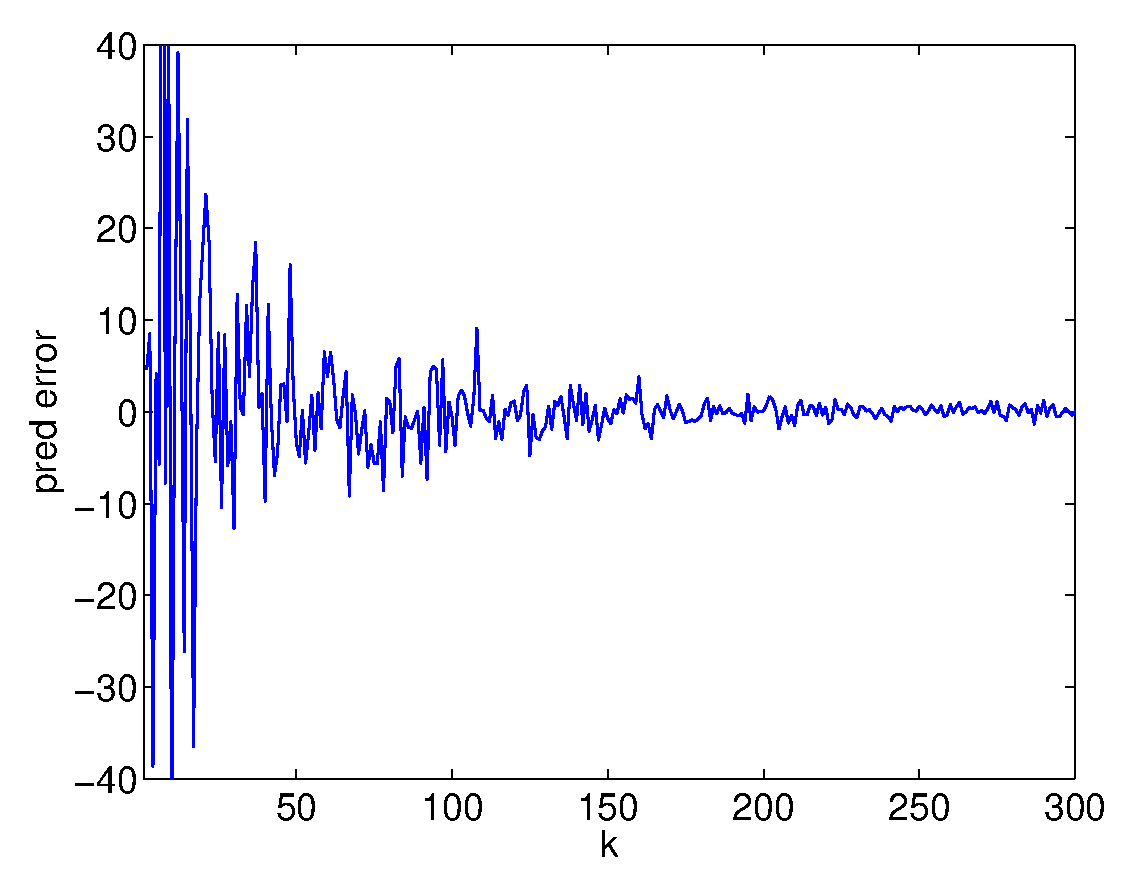
\includegraphics[width=0.65\textwidth]{matlab/online_reg_errors}
\end{center}
\caption{Prediction error $w^{(k)T}x^{(k+1)}-y^{(k+1)}$
versus iteration number $k$.}
\label{f-online-reg-errors}
%\end{figure}
%
%\begin{figure}
\begin{center}
\psfrag{sign}[][]{}
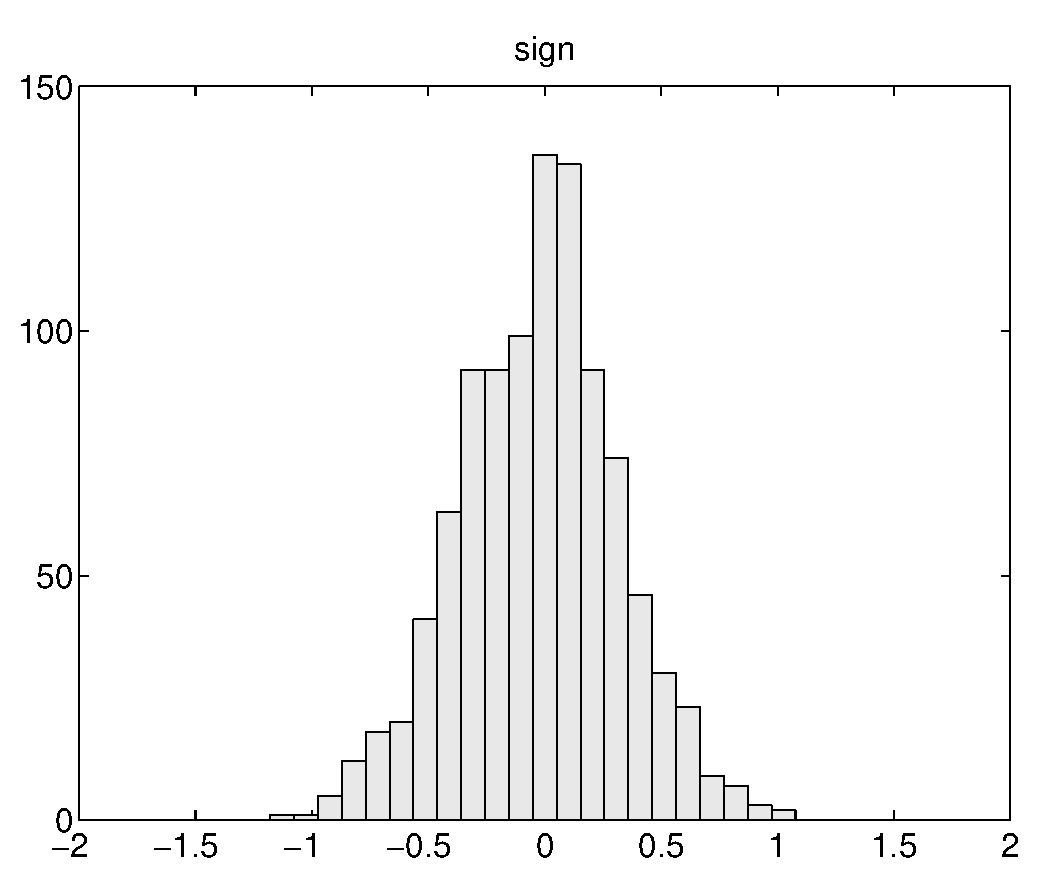
\includegraphics[width=0.65\textwidth]{matlab/online_reg_dist}
\end{center}
\caption{Empirical distribution of prediction errors
for $w^\star$, based on $1000$ samples.}
\label{f-online-reg-dist}
\end{figure}

\iffalse
\subsection{Least mean squares (LMS) algorithm}

We consider the problem of adaptively choosing weights
$w \in \reals^n$ of an FIR filter in order to minimize
the mean-square error between the filter output
$w^T x \in \reals$ and the reference signal~$y \in \reals$.
Here $x\in\reals^n$ are the $n$~current samples of the input
signal $x(t)$. Note that the problem setup is the same
as the one of the on-line learning and regression.

Here we have the mean-square loss function $l(u) = u^2$,
and derive an update rule for the weights based on
a noisy (unbiased) subgradient
\begin{eqnarray*}
w^{(k+1)} & = & w^{(k)}-\alpha_k
l'(w^{(k)T}x^{(k+1)}-y^{(k)})x^{(k+1)} \\
& = & w^{(k)}-\alpha_k
2(w^{(k)T}x^{(k+1)}-y^{(k)})x^{(k+1)} \\
& = & w^{(k)} - 2\alpha_k
\left( x^{(k+1)} x^{(k+1)T}w^{(k)}
- y^{(k)}x^{(k+1)} \right).
\end{eqnarray*}

In the case when we know the mean and covariance matrix of $(x,y)$,
we can derive an analytic formula for the optimal $w$,
since we can compute the gradient of the mean-square loss function,
\ie,
\[
\nabla J(w) = 2\Expect x x^T w - 2 \Expect yx,
\]
and
\[
w^\star = (\Expect x x^T)^{-1} \Expect yx.
\]
(or i guess we really need to use autocorrelation
and cross-correlation functions ...)

We can also obtain the optimal $w$ by applying
the subgradient update
\begin{eqnarray*}
w^{(k+1)} & = & w^{(k)} - 2\alpha_k
\left( \Expect x x^T w^{(k)}
- \Expect yx \right).
\end{eqnarray*}
Given a fixed stepsize $\alpha_k = \alpha$,
this is the famous \emph{least mean squares} (LMS)
algorithm proposed by Widrow and Hoff.
If the covariance matrices are not known, they can
be estimated in the process (sampled covariances).

\begin{itemize}
\item i guess that RLS, LMS, and sign algorithms
for plant-identification and signal tracking
can all be put into this framework ...

\item there are many variations of the LMS algorithm
such as averaged LMS, momentum LMS, \etc,
that is exactly what we have talked about in trying to
speed-up the subgradient method

\item for example, define error $e = ( w^T x - y )$,
we can write ``leaky'' LMS update as
\[
w^{(k+1)} = (1 - \mu) w^{(k)} - 2\mu \alpha_k e^{(k)}x^{(k)}
\]
where $\mu > 0$ is the leakage parameter

this is a simple `filtered' version of the stochastic
subgradient method

\item
it looks like the ``sign'' algorithm minimizes
\[
J(w) = \Expect \| w^T x - y \|_1
\]
define error $e = ( w^T x - y )$,
a noisy (unbiased) subgradient is
$\tilde g = \sign(e)x$

then the update of the sign algorithm is
\[
w^{(k+1)} = w^{(k)} - \alpha_k \sign(e^{(k)}) x^{(k)}
\]

\item in normalized LMS, the noisy subgradient step
is normalized by the energy of the data vector, \ie,
we have update
\[
w^{(k+1)} = w^{(k)} - \frac{\alpha_k}{\|x^{(k)}\|_2^2}
2 e^{(k)} x^{(k)}
\]
where we define error signal as $e = ( w^T x - y )$,
and often one uses step size rules like
\[
\frac{\alpha_k}{a + \|x^{(k)}\|_2^2}
\]
to overcome numerical instability when $\|x^{(k)}\|_2$
is close to zero
\end{itemize}
\fi


\section*{Acknowledgments}

May Zhou helped with a preliminary version of this document.
We thank Abbas El~Gamal for helping us simplify the convergence proof.
Trevor Hastie suggested the on-line learning example.

\bibliography{subgrad_method}

\end{document}
